\section{CMMI - Capabilty Maturity Model Integration}
Il \textbf{Capability Maturity Model Integration (\textit{CMMI})} è un programma di formazione e valutazione per il miglioramento a livello di processo gestito dal \textit{CMMI Institute}.\\ 
Bisogna prima introdurre il concetto di \textbf{maturità dei processi}. 
La probabilità di portare a termine un progetto dipende dalla \textit{maturità del progetto} e la maturità dipende dal grado di controllo che si ha sulle azioni che si vanno a svolgere per realizzare il progetto. 
Si ha quindi che: 
    \begin{itemize} \item il progetto è \textbf{immaturo} quando le azioni legate allo sviluppo non sono ben definite o ben controllate e quindi gli sviluppatori hanno troppa libertà che rischia di degenerare in una sorta di anarchia nel controllo del processo di sviluppo, alzando la probabilità di fallimento 
    \item il progetto è \textbf{maturo} quando le attività svolte sono ben definite, chiare a tutti i partecipanti e ben controllate. Si ha quindi un modo per osservare quanto si sta svolgendo e verificare che sia come pianificato, alzando le probabilità di successo e riducendo quelle di fallimento.
\end{itemize}

La \textbf{maturità del processo} è definita tramite un insiemi di livelli di maturità con associate metriche per gestire i processi, questo è detto \textbf{Capability Maturity Model (\textit{CMM})}. In altri termini il modello CMM è una collezione dettagliata di \textit{best practices} che aiutano le organizzazioni a migliorare e governare tutti gli aspetti relativi al processo di sviluppo.
%%% foto del diagramma 
\begin{figure}[H]
    \centering
    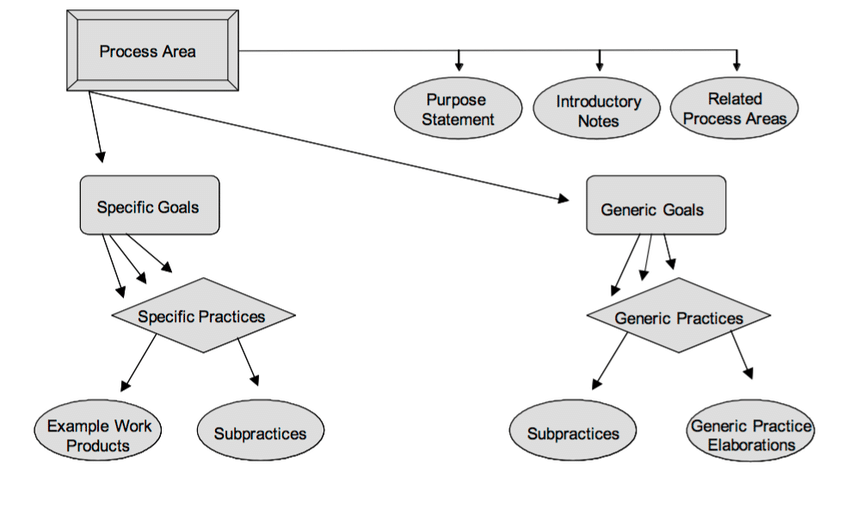
\includegraphics[scale = 0.4]{Imm/CMMI-Dev-Model-components-in-Tea10.png}
    \label{fig:my_label}
\end{figure}
All'interno del diagramma notiamo: 
\begin{itemize} 
    \item \textbf{Process area}, che racchiude al suo interno una collezione di pratiche organizzate secondo obiettivi, e riguarda una certa area del processo di sviluppo software. Nel CMMI abbiamo 22 diverse \textit{process area}, tra cui \textit{configuration management}, \textit{project planning}, \textit{risk management}, $\dots$. Nel diagramma si ha lo studio di una generica \textit{process area}, ciascuna \textbf{process area} ha: 
        \begin{itemize} 
            \item un \textbf{purpose statement}, che descrive lo scopo finale della \textit{process area} stessa 
            \item un \textbf{introductory notes}, con nel note introduttive che descrivano i principali concetti relativi alla \textit{process area} 
            \item un \textbf{related process area}, che contiene la lista delle altre \textit{process area} correlate a quella corrente, se presenti.
        \end{itemize} 
    \item le \textbf{process area} si dividono in due \textit{tipologie di obiettivi}: 
        \begin{enumerate} 
            \item \textbf{specific goals}, ovvero gli obiettivi specifici della singola \textit{process area} in questione. Questi obiettivi caratterizzano la \textit{process area} 
            \item \textbf{generic goals}, ovvero gli obiettivi comuni a \textbf{tutte} le \textbf{process area}. Questi obiettivi rappresentano quanto la \textit{process area} sia ben integrata e definita nel contesto del processo ma questi criteri sono generali 
        \end{enumerate} 
    \item all'interno di ogni \textbf{specific goals} abbiamo una serie di \textbf{specific practices}, ovvero quelle azioni che se svolte permettono di raggiungere quell'obiettivo specifico e, a loro volta, tali pratiche sono organizzate in: 
        \begin{itemize} 
            \item \textbf{example work product}, ovvero elenchi di esempi di prodotti che possono essere generati attraverso l'adempimento delle pratiche 
            \item \textbf{subpractices}, ovvero pratiche di grana più fine
        \end{itemize} 
    \item all'interno di ogni \textbf{generic goals} abbiamo una serie di \textbf{generic practices} comuni a tutti, con le pratiche che devono essere svolte per gestire opportunamente una qualsiasi \textit{process area} e a loro volta tali pratiche sono organizzate in: 
        \begin{itemize} 
            \item \textbf{generic practices elaborations}, ovvero ulteriori informazioni di dettaglio per la singola pratica
            \item \textbf{subpractices}, ovvero pratiche di grana più fine 
        \end{itemize} 
\end{itemize}

Per capire quanto bene un processo software è organizzato secondo questo standard bisogna mappare quali goals e quali pratiche si stanno perseguendo e seguendo e usare CMMI non solo come ispirazione, ma come vero e proprio \textbf{standard} per definire le azioni da svolgere nonché per confrontare il nostro operato e studiarlo qualitativamente. Lo studio qualitativo mi permette di stabilire la \textbf{maturità} del progetti, secondo un certo livello di \textit{compliance}, detto \textbf{CMMI level}. Tale qualità che può essere certificata da enti certificatori appositi.\\

Ci sono due linee di sviluppo, rispetto a questo standard, che bisogna prendere in considerazione:
\begin{enumerate}
    \item \textbf{capability levels (\textit{CL})}, che cattura e rappresenta quanto bene si sta gestendo una particolare \textit{process area} (quindi ciascuna \textit{process area} può raggiungere un diverso CL). Quindi per una singola \textit{process area} mi dice quanto bene sto raggiungendo i \textit{generic goals} (e di conseguenza anche i vari \textit{specific goals}, in quanto quelli generici impongono il controllo e la documentazione di quelli specifici). 
    Il CL ha valore da 0 a 3: 
        \begin{itemize} 
            \item \textbf{level 0: \textit{incomplete}}, dove probabilmente non si stanno nemmeno svolgendo tutte le pratiche richieste per quella \textit{process area} o sono state svolte solo parzialmente 
            \item \textbf{level 1: \textit{performed}}, dove si eseguono le pratiche e i vari \textit{specific goals} sono soddisfatti 
            \item \textbf{level 2: \textit{managed}}, dove oltre alle pratiche si ha anche una gestione delle attività stesse, come indicato nello standard.
            \item \textbf{level 3: \textit{defined}}, dove l'intero processo è ben definito secondo lo standard, descritto rigorosamente e si ha un processo completamente su misura dell'organizzazione 
        \end{itemize} 
    I CL di ciascuna \textit{process area} possono essere rappresentate su un diagramma a barre, dove viene indicato il CL attuale e il \textbf{profile target}, ovvero il livello a cui quella \textit{process area} deve arrivare (che non è per forza il terzo). 
    
    \item \textbf{maturity levels (\textit{ML})}, che cattura il livello raggiunto dall'intero processo di sviluppo ragionando su tutte le \textit{process area} che sono state attivate. Rappresenta quanto bene si sta lavorando sull'insieme intero della \textit{process area}. 
    A livello di grafico punta direttamente all'elemento specificante la \textit{process area}. Il ML ha valore da 1 a 5: 
        \begin{itemize} 
            \item \textbf{level 1: \textit{initial}}, dove si ha un processo gestito in modo caotico, scarso controllo
            \item \textbf{level 2: \textit{managed}}, dove si ha già un processo ben gestito secondo varie policy 
            \item \textbf{level 3: \textit{defined}}, dove si ha un processo ben definito secondo lo standard aziendale 
            \item \textbf{level 4: \textit{quantitatively managed}}, dove si stanno anche raccogliendo dati che misurano quanto bene sta andando bene il processo, facendo quindi una misura quantitativa dello stesso 
            \item \textbf{level 5: \textit{optimizing}}, dove grazie alle informazioni raccolte nel livello precedente ottimizzo il processo, in un'idea di \textit{continuous improvement} del progetto stesso 
        \end{itemize} 
    Gli ultimi due livelli sono davvero difficili da raggiungere.
\end{enumerate}

Tra i principali \textit{generic goals (GG)} abbiamo: 
\begin{itemize} 
    \item \textit{GG1}: raggiungere i \textit{specific goals}, tramite l'esecuzione delle \textit{specific practices} 
    \item \textit{GG2}: ufficializzare un \textit{managed process}, tramite training del personale, pianificazione del processo, controllo dei \textit{work product}, $\dots$ 
    \item \textit{GG3}:  ufficializzare un \textit{defined process}, tramite la definizione rigorosa del progetto e la raccolta di esperienze legate al processo 
\end{itemize}